% !TEX TS-program = pdflatex
% !TEX root = ../LightMicroRep.tex

%************************************************
\chapter{Laser Scanning Microscopy}
\label{chp:LSM}
%************************************************
\numberwithin{figure}{section}
%----------------------------------------------------------------------------------------
%	INTRODUCTION
%----------------------------------------------------------------------------------------

\section{Introduction}

\paragraph{Aim (Basic)}To get to know basic Laser Scanning Microscopy (LSM) functions.
\paragraph{Aim (Multifluorescence)}To investigate multifluorescent specimens, spectral analysis, and 3-D imaging.
\\

Confocal Laser Scanning Microscopy (Confocal LSM/CLSM/Confocal/LSM) is a high-resolution optical imaging technique. 
This technique utilizes a pinhole at the focal point to remove fluorescence emissions originating from planes other than the one in focus, although regions that do not directly contribute to the useful signal are still exposed to excitation light, which may lead to photodamage.

It works by acquiring fluorescence signal in a scanning manner, i.e. point-by-point in a line, and line-by-line in a plane to produce a high resolution 2D image. 
Since this imaging technique results in a very thin slice of image (axially), imaging different planes and combining them can produce a 3D image of a specimen.

%----------------------------------------------------------------------------------------
%	METHODS
%----------------------------------------------------------------------------------------

\section{Methods}

\subsection{Basic LSM}
To familiarize basic LSM functions, several images of the rhizome of lily of the valley specimen were taken.  
Most images were taken using the objective lens EC Epiplan Neofluar 20$\times$/0.5 DIC M27, unless otherwise stated. Obtained images were then coded in 16 bits and then compared to observe the effect of different pinhole sizes, scanning speeds, laser intensities, NA, and digital resolutions.

\subsection{Multifluorescence, Spectral Analysis, and 3-D Imaging}
Several different specimens are investigated in this section, namely: bovine endothelial cells, cross section of the rhizome of Lily of the valley, algae and diatomes, cells from a blowfly's abdomen, blowfly salivary gland, and a gold covered coverslip. 
The particular techniques are discussed in the following section in more detail. 
The objective lenses used are: Plan-Apochromat 63$\times$/1.4 Oil, Plan-Neofluar 20$\times$/0.5, and C-Apochromat $\times$/1.2 lmm. 
Full-Width at Half-Maximum (FWHM) calculations are done in \faPython Python (script available publicly on \href{https://github.com/howset/LightMicro}{\faGithub~GitHub}, or by request).

%----------------------------------------------------------------------------------------
%	RESULTS AND DISCUSSION
%----------------------------------------------------------------------------------------
\section{Results and Discussion}

%----------------------------------
\subsection{Basic LSM}

\begin{figure}[h!]
\centering
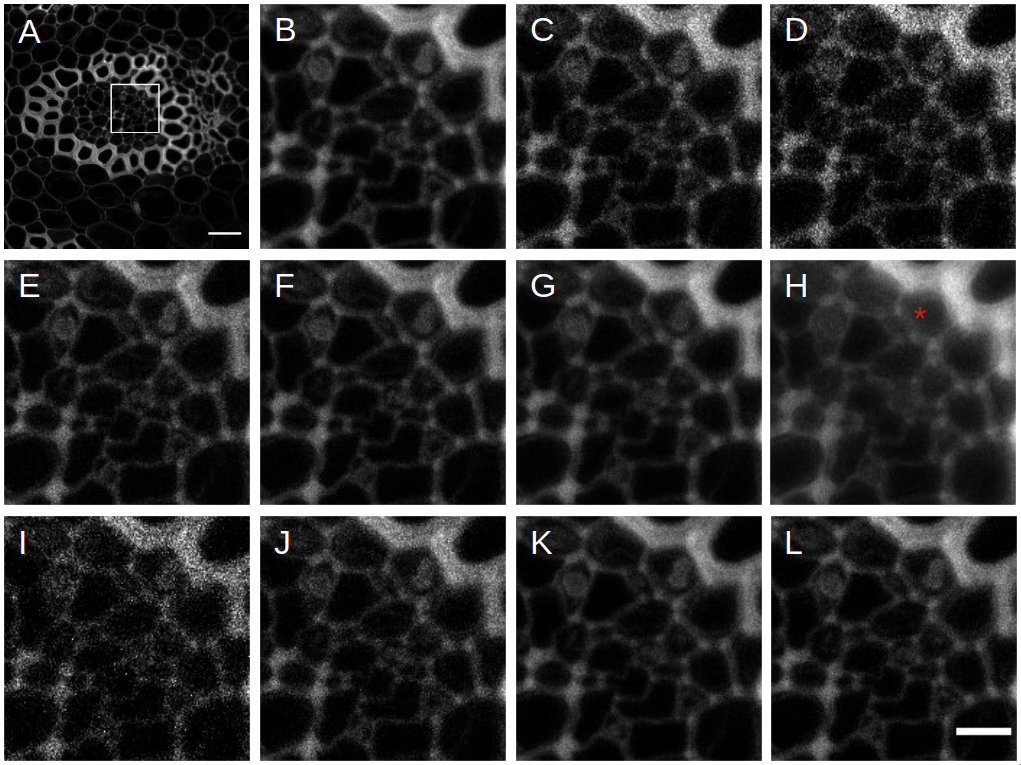
\includegraphics[width=\columnwidth]{Exp_3_LSM/Figures/Bcr/LSMmergedv2}	
\caption[different scanspeed]{Lily of the valley specimen. \textbf{A}: original image with white square marking the magnified area. 
\textbf{B-D} are the sample imaged with varying scanning speed, \textbf{E-H} with varying pinhole sizes, \textbf{I-L} with varying laser intensity. 
B: Minimum scanspeed, C: Medium scanspeed, D: Maximum scanspeed. 
E: Pinhole 0.5 AU, F: Pinhole 1 AU, G: Pinhole 2 AU, H: Pinhole maximum. 
I: Laser 0.5, J: Laser 2, K: Laser 2 (with averaging 4), L: Laser 5. 
Objective lens: EC Epiplan Neofluar 20$\times$/0.5 DIC M27. 
Scalebar on original image is 30 $\mu$m, on the zoomed in image is 10 $\mu$m. 
Red asterisk shows the disappearance of the small structure.} 
\label{fig:LSMmerged}
\end{figure}

To compare how different scanning speed may have influence on imaging, imaging was done using different scanning speeds. 
Fig.~\ref{fig:LSMmerged}B-D shows the effect of scanning speed of Lily of the valley specimen (Fig.~\ref{fig:LSMmerged}A). 
As can be seen, slower scanning speed allows for a higher resolution image and increasing the scanning speed reduces the resolution of an image and makes the zoomed-in image heavily pixelated, however this also makes the imaging process faster. 
A slower scanning speed could be advantageous in yielding a higher resolution image, however this increases the time necessary to conduct the imaging and also the risk of photobleaching the specimen. 

The pinhole is a hallmark of a confocal microscopy system, it allows for the removal of emissions that do not come from the focal plane. 
The size of the pinhole generally should be exactly the size of the Airy disc \cite{LeicaMicro}, given in Airy Units (AU). 
Enlarging the pinhole allows for more extrafocal contribution to reach the detector, increasing the blurriness by signals from other planes. 
Decreasing the size would in theory allow the minimal extrafocal signal, and hence the thinnest focal plane. 
But closing the pinhole would defeat the purpose of imaging afterall. 
The effect of different pinhole sizes can be seen in Fig.~\ref{fig:LSMmerged}E-H. 
Larger pinhole makes image more blurry due to the reason mentioned before. 
The blurriness would hinder proper identification of structures as pointed by the red asterisk in Fig.~\ref{fig:LSMmerged}H. 

Shown in Fig.~\ref{fig:LSMmerged}I-L are the images taken with different laser intensity (0.5, 2, 2 with averaging, and 5). 
The intensity of laser to use during imaging depends on the specimen being imaged and the setting of the imaging device. 
A sensitive specimen may not be able to be subjected to high intensity laser, which may destroy fluorescent species or the structure itself. 
A low intensity laser, on the other hand, may not produce enough energy to be detected by the light detector in the device. 
For this, the gain setting (amplification of input signal - increase the brightness of light features) and offset setting (zeroing the background level - set the darkest part to black) has to be set properly to compensate the weak signal to the surrounding noise (Signal to Noise ratio - SNR). 
Hence, for sensitive specimen, a low intensity laser that does not destroy the specimen would require a compensating gain and offset setting. 
The SNR in this case may not be the best. 

Comparing the images taken using laser intensity 2 with and without averaging (Fig.~\ref{fig:LSMmerged}J\&K) shows the effect of it. 
The particular function takes the average of a longer sampling time when imaging. 
A longer sampling time (more signal acquisition), or higher averaging level would lead to better SNR because more frames are gathered and averaged. 
This is evident from (Fig.~\ref{fig:LSMmerged}K\&L) where averaging gives a clearer image with a lot less noise than without. 
Since the Lily of the valley specimen used in this experiment autofluoresce and almost impossible to bleach, a higher averaging level would be preferable to obtain a smoother image. 
But otherwise, for more sensitive specimen, a longer sampling time may be disadvantageous. 

\begin{figure}[h!]
\centering
\subfloat[Magnification 10$\times$\label{m10x}]{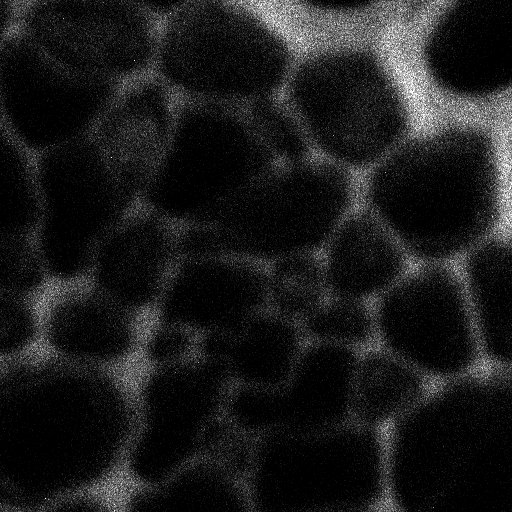
\includegraphics[width=.28\columnwidth]{Exp_3_LSM/Figures/Bcr/Task5_10x_t}}\hspace{0.1em}
\subfloat[Magnification 20$\times$\label{m20x}]{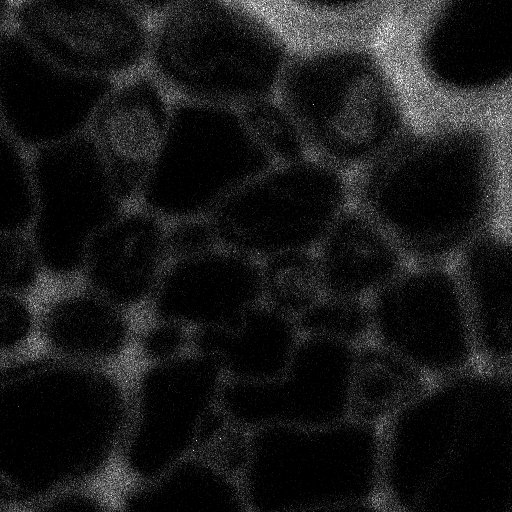
\includegraphics[width=.28\columnwidth]{Exp_3_LSM/Figures/Bcr/Task5_20x_t}}\hspace{0.1em}
\subfloat[Magnification 40$\times$\label{m40x}]{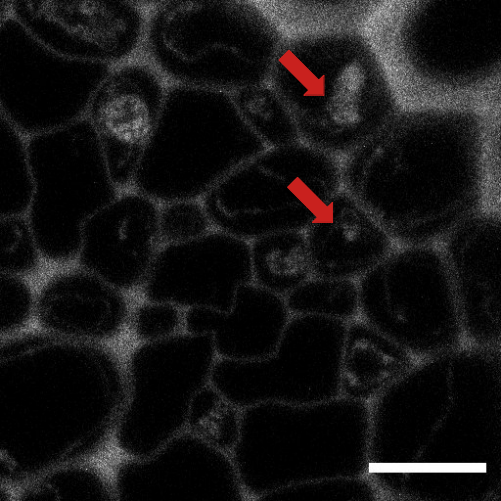
\includegraphics[width=.28\columnwidth]{Exp_3_LSM/Figures/Bcr/Task5_40x_t_10um10_edited4}}\\
\caption{Lily of the valley specimen imaged using different magnification on the same image plane. 
Digital resolution of original images are 1024$\times$1024. 
Shown here are insets corresponding to the image in Fig.~\ref{fig:LSMmerged}A. Objective lens: A: EC Plan neofluar 10$\times$/0.3 M27, B: EC Epiplan Neofluar 20$\times$/0.5 DIC M27, C: EC Plan neofluar 40$\times$/1.3 Oil DIC. 
Scalebar is 10 $\mu$m. Red arrows show smaller structures that are visualized more clearly.}
\label{fig:LSMmag}
\end{figure}

Fig.~\ref{fig:LSMmag} shows the effect of different magnifications on a sample. 
It can be observed that higher magnification yields better imaging result for smaller structures, demonstrated visually in Fig.~\ref{m40x} with the smaller structures shown more clearly pointed by the red arrows. 
The magnification is a property of the utilized objective lens and is strongly related to the NA. 
The higher the NA of a lens, the clearer an image is. 
The NA is, however, determined by the refractions index and angle of the cone of light. 
To increase the NA, and hence the optical resolution, a higher refractions index is desireable. 
This can be achieved by using a different medium (NA$_{air} \approx$ 1, NA$_{water} \approx$ 1.3, NA$_{oil} \approx$ 1.5; depending on $\lambda$). 
Of course, the objective must be suitable for the preferred medium.

\begin{figure}[h!]
\centering
\captionsetup[subfigure]{position=top}
\subfloat[Original image\label{ori}]{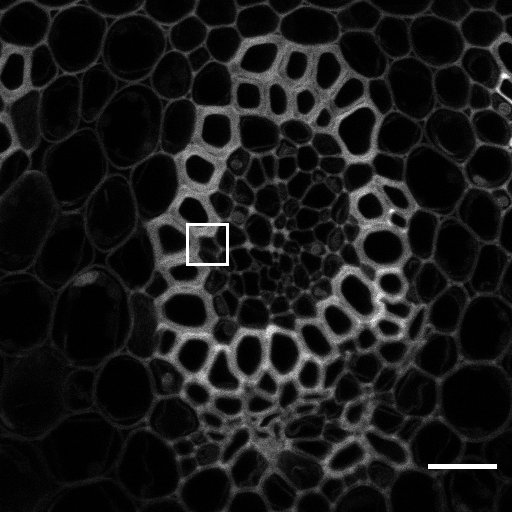
\includegraphics[width=.28\columnwidth]{Exp_3_LSM/Figures/Bcr/Task1_Group3_forres_30um5}}\hspace{0.1em}
\subfloat[$256\times256$\label{res256}]{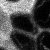
\includegraphics[width=.28\columnwidth]{Exp_3_LSM/Figures/Bcr/Task6_256}}\hspace{0.1em}
\subfloat[$512\times512$\label{res512}]{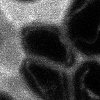
\includegraphics[width=.28\columnwidth]{Exp_3_LSM/Figures/Bcr/Task6_512}}\vspace{-0.7em}
\captionsetup[subfigure]{position=bottom}
\subfloat[$860\times860$\label{res860}]{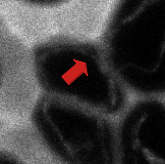
\includegraphics[width=.28\columnwidth]{Exp_3_LSM/Figures/Bcr/Task6_860optimal_edited3}}	\hspace{0.1em}
\subfloat[$1024\times1024$\label{res1024}]{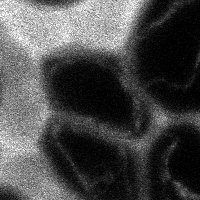
\includegraphics[width=.28\columnwidth]{Exp_3_LSM/Figures/Bcr/Task6_1024}}\hspace{0.1em}
\subfloat[$2048\times2048$\label{res2048}]{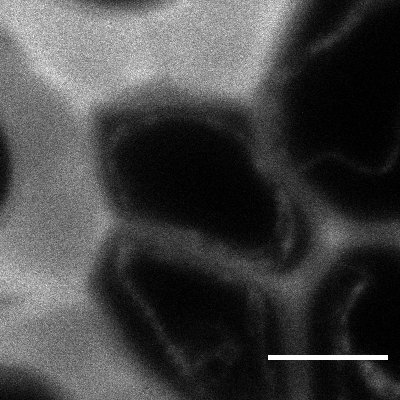
\includegraphics[width=.28\columnwidth]{Exp_3_LSM/Figures/Bcr/Task6_2048_5um5}}\\
\caption{Lily of the valley specimen pictured with different digital resolutions. 
White square on the original image marks the magnified area. 
Objective lens: EC Plan neofluar 40$\times$/1.3 Oil DIC. Scalebar on original image is 30 $\mu$m, on the zoomed in image is 5 $\mu$m. 
Thick red arrow shows smaller structures that can be distinguished more clearly.} 
\label{fig:LSMres}
\end{figure}

The effect of different image (digital) resolution can be seen in Fig.~\ref{fig:LSMres}. 
The optical resolution of a digital image depends on the sampling interval to make an accurate representation of the real features of a specimen. 
To maintain the spatial resolution of an image, according to Nyquist criterion, the sampling interval has to be equal to twice the highest spatial frequency of the specimen \cite{ZeissCamp}. 
Any lower than this, then features with higher spatial frequency will not be readily resolvable, as shown by the red arrow in Fig.~\ref{res860}, which shows a smaller structure that can start to be resolved on a digital resolution at least $512\times512$ (more clearly seen on $860\times860$), which would otherwise be unresolved (indistinguishable with neighbouring structures) on resolutions lower than that. 
For live cell imaging sessions however, the Nyquist criterion may have to be violated in order to maintain the well being of the specimen.

\begin{figure}[h]
\centering
\subfloat[MIP\label{bmip}]{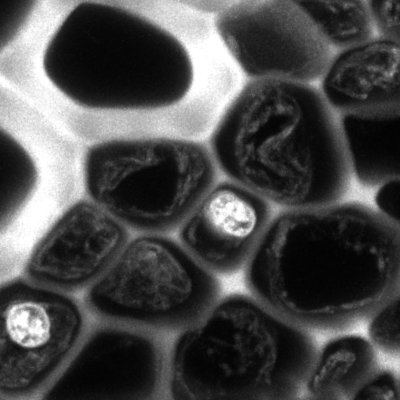
\includegraphics[width=.3\columnwidth]{Exp_3_LSM/Figures/Bcr/Task7_z-stack_MIP_cropped}}\hspace{0.1em}
\subfloat[3D\label{3d}]{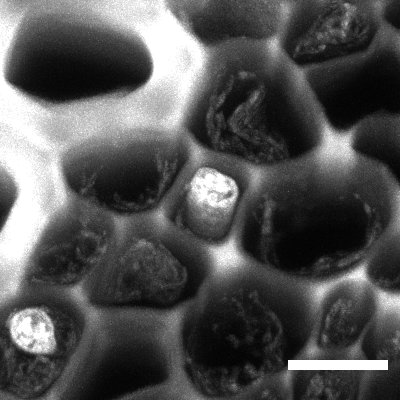
\includegraphics[width=.3\columnwidth]{Exp_3_LSM/Figures/Bcr/Task7_z-stack_3Dpicture_cropped_10um10}}\\
\caption{Lily of the valley specimen, Maximum intensity projection and 3D picture (one perspective). 
Objective lens: EC Plan-Neofluar 40$\times$/1.3 Oil DIC. 
Scalebar is 10 $\mu$m.} 
\label{fig:LSMmip3d}
\end{figure}

Fig.~\ref{bmip} shows the Maximum Intensity Projection (MIP) of the sample. 
The maximum intensity projection results in a brighter and clearer image of every structure because it adds the intensity of every layer of the stacked images. 
As mentioned before, the confocal technique allows for optical sectioning, in which a specimen can be imaged layer-by-layer along the axial- or z-axis. 
The combined result of this layer-by-layer imaging produces a 3D image of the specimen. 
Fig.~\ref{3d} shows one perspective of the acquired image. 
This image is obtained by making a so-called z-stack acquisition of the specimen. 

%----------------------------------------------------------------------------------------------------
\subsection{Multifluorescence, Spectral Analysis, and 3-D Imaging}

Some investigations may require multiple labelling of a specimen to observe different parts of the cell and it is advantageous to simultaneously image this multiply labelled specimen in contrast to doing it sequentially. 
However, problems may arise due to signal interference (also called crossover, bleed-through, or crosstalk) when the fluorescence signal is close to each other. 
This phenomenon is demonstrated in Fig.~\ref{fig:bovendo} that shows multiply labelled bovine endothelial cells. 
The top row shows imaging in single track mode, where DAPI signal bleeds through to AlexaFluor488-Phalloidin channel (Fig.~\ref{fig:bovendo}A-C) but not to the Mitotracker channel. 
This is confirmed by removing the excitation on 405 nm (Fig.~\ref{no405}) where the bleed-through is removed. 
Some strategies can be employed in approaching such a problem, namely by means of mathematical approach that involves applying algorithms termed \textit{channel unmixing} \cite{NikonMicro}\cite{Lect11}. 
This method does not really work because the algorithm functions on where the intensity is the highest, and in this case, it is on where the nucleus is, therefore it is necessary to decrease DAPI excitation. 
The result can be seen in Fig.~\ref{unmix} where the bleed-through is significantly reduced although some traces can still be recognized along with some dark spots that seems to trace the mitotracker signal. 
Another approach is by using multitracking option to enable fast switching between laser lines using an acousto-optic tunable filter (AOTF) to separate excitation (and the subsequent gathering of fluorescence emission) of each fluorophore \cite{ZeissCamp3}. 
The result in Fig.~\ref{multt} shows no bleed-through that can be observed.

\begin{figure}[h!]
\centering
\captionsetup[subfigure]{position=top}
\subfloat[DAPI\label{D}]{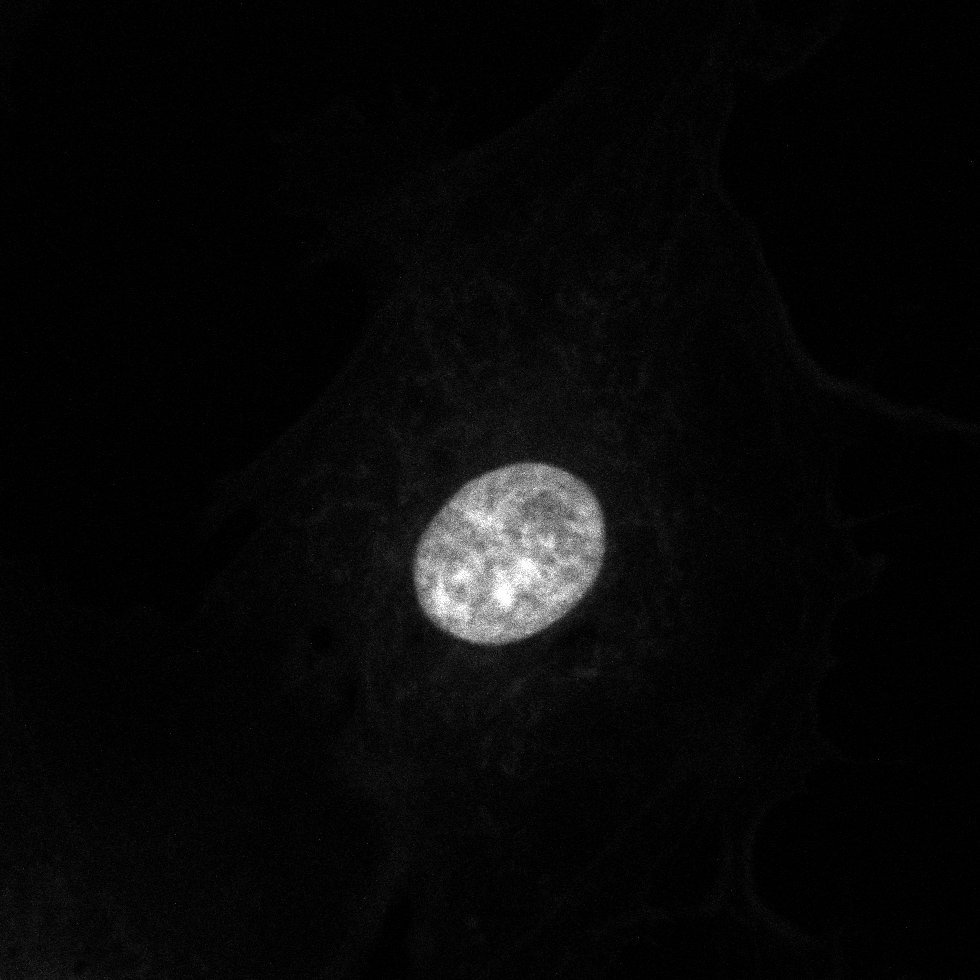
\includegraphics[width=.28\columnwidth]{Exp_3_LSM/Figures/MS3/F1-C1-task1a2}}\hspace{0.1em}
\subfloat[AlexaFluor488\label{P}]{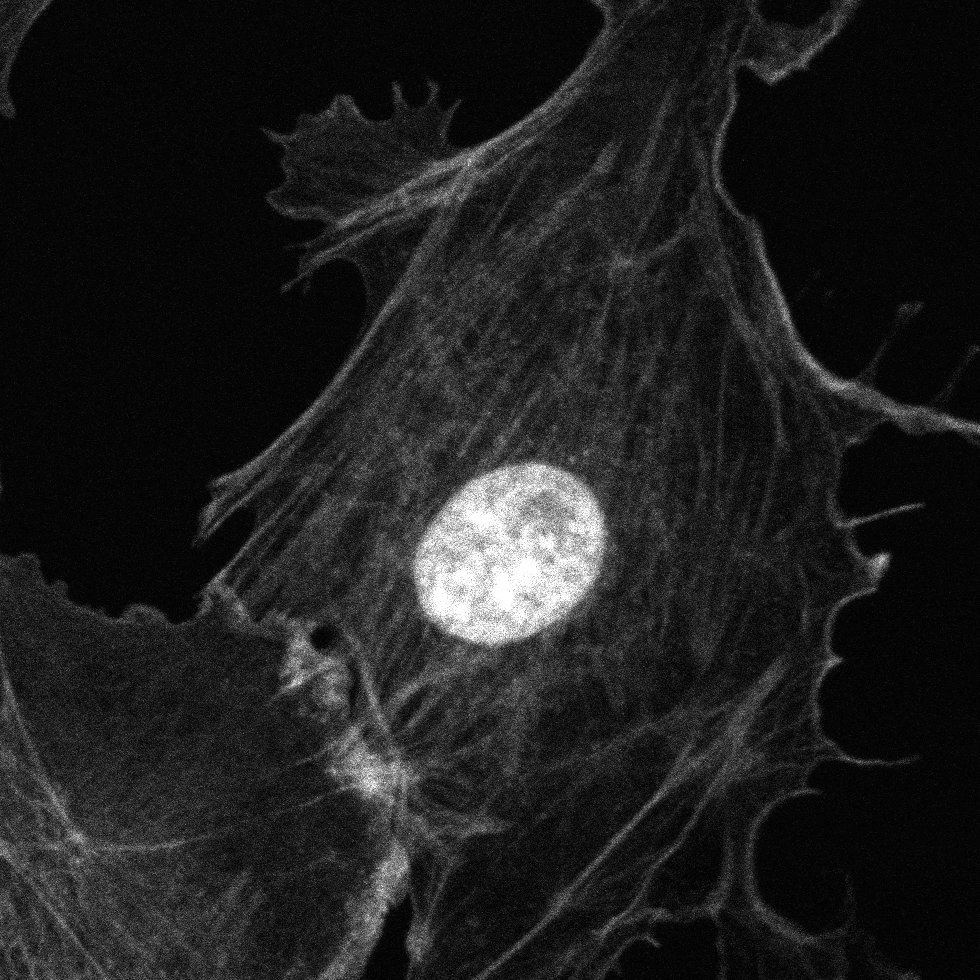
\includegraphics[width=.28\columnwidth]{Exp_3_LSM/Figures/MS3/F1-C2-task1a2}}\hspace{0.1em}
\subfloat[Mitotracker\label{M}]{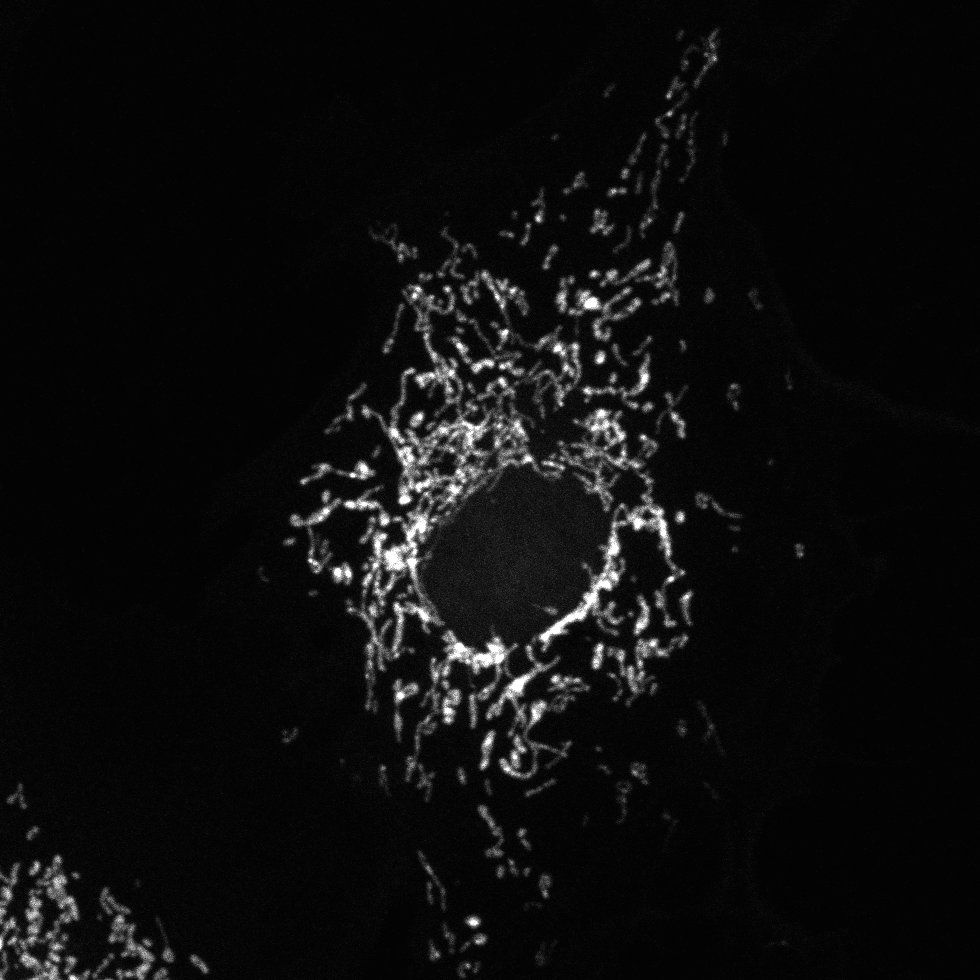
\includegraphics[width=.28\columnwidth]{Exp_3_LSM/Figures/MS3/F1-C3-task1a2}}\vspace{-0.7em}
\captionsetup[subfigure]{position=bottom}
\subfloat[no 405 nm exc.\label{no405}]{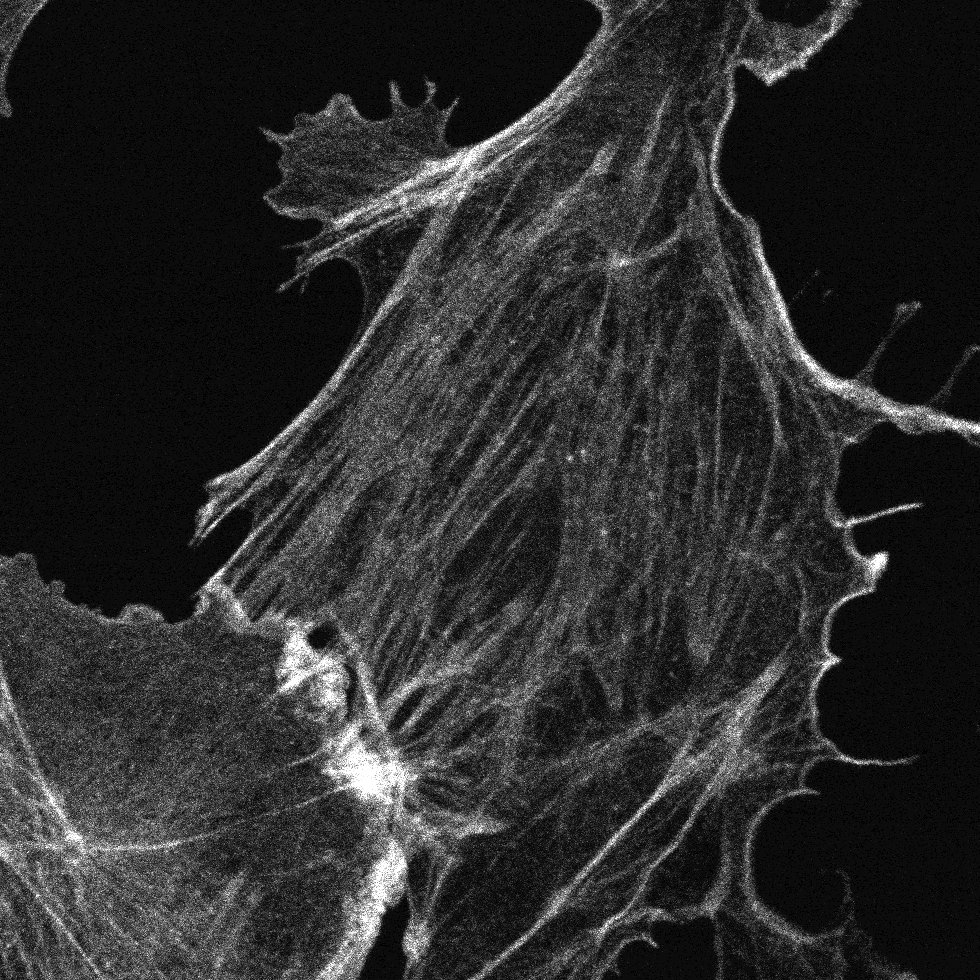
\includegraphics[width=.28\columnwidth]{Exp_3_LSM/Figures/MS3/F1-C2-task1a_no405}}	\hspace{0.1em}
\subfloat[Channel Unmixing\label{unmix}]{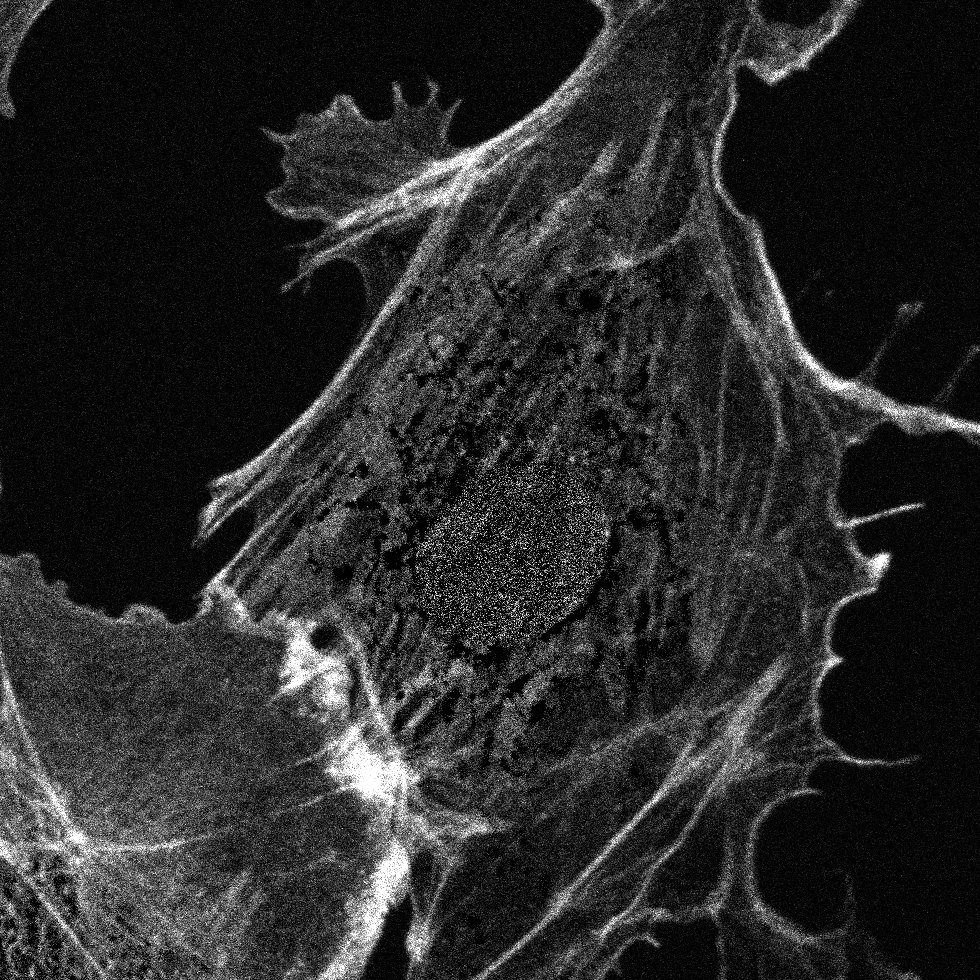
\includegraphics[width=.28\columnwidth]{Exp_3_LSM/Figures/MS3/F1-C2-task1a2_Linear unmixing}}\hspace{0.1em}
\subfloat[Multitrack\label{multt}]{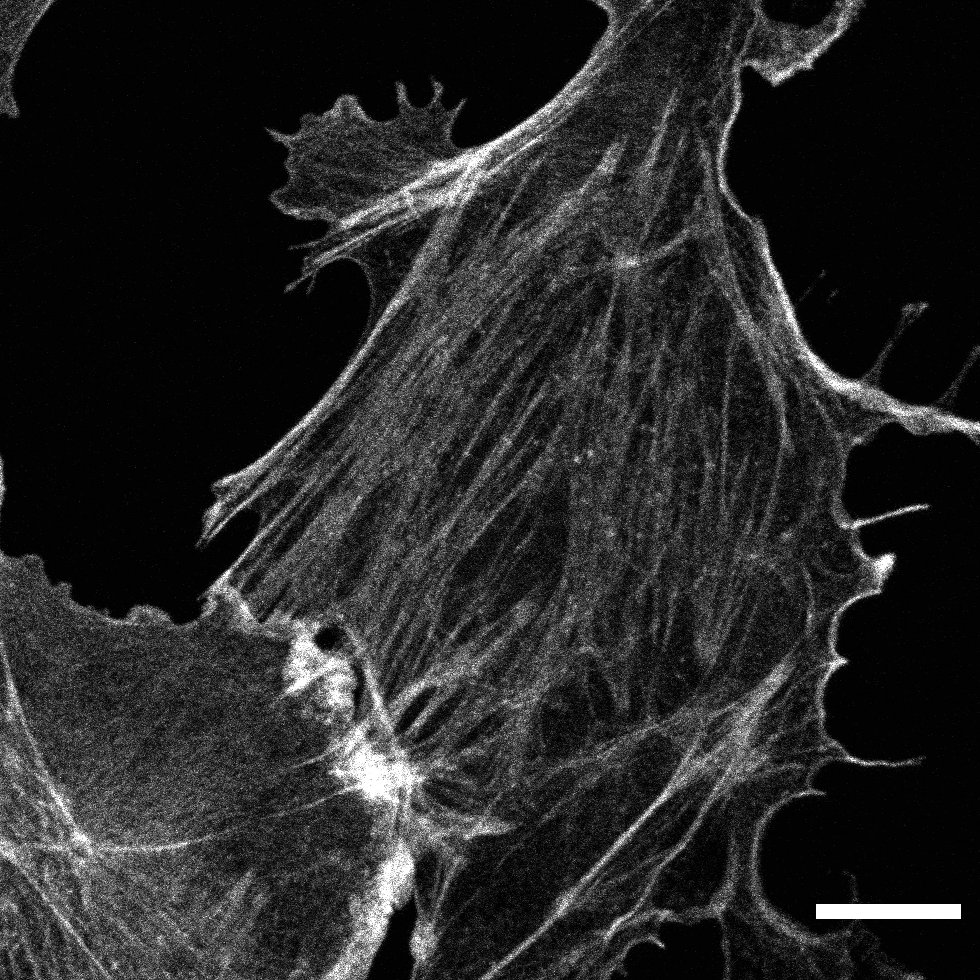
\includegraphics[width=.28\columnwidth]{Exp_3_LSM/Figures/MS3/F1-C3-task1d_10um}}\\
\caption{Top row: 3 channels of bovine endothelial cells image acquisition labelled by: DAPI that binds to the nucleus, AlexaFluor 488-Phalloidin that binds to the actin filaments, and Mitotracker RedCMXRos that binds to mitochondria using single track acquisition. 
Bottom row: Images of the channel AlexaFluor488: without 405 nm excitation, using channel unmixing, and multi-tracking. 
Objective lens: Plan Apochromat 63$\times$/1.4 Oil. 
Scalebar is 10 $\mu$m.} 
\label{fig:bovendo}
\end{figure}

\begin{figure}[h!]
\centering
\subfloat[Channels \& Emission Spectra\label{ES}]{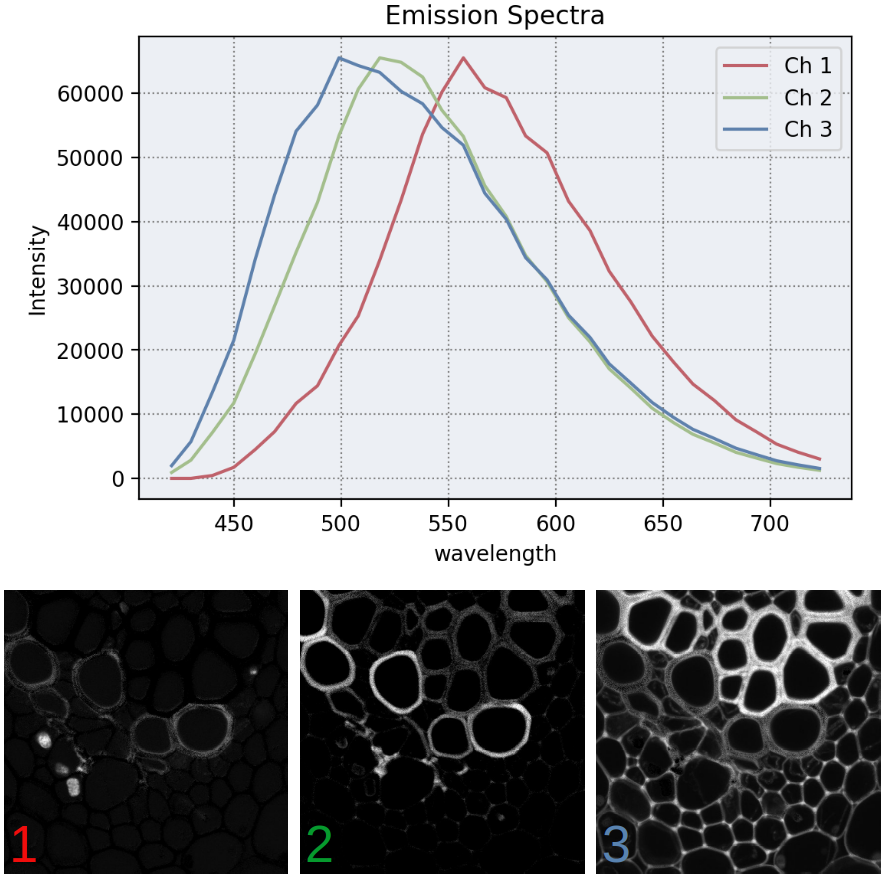
\includegraphics[width=.49\columnwidth]{Exp_3_LSM/Figures/MS3/F2_grey1}}\hspace{0.1em}
\subfloat[Composites\label{Co}]{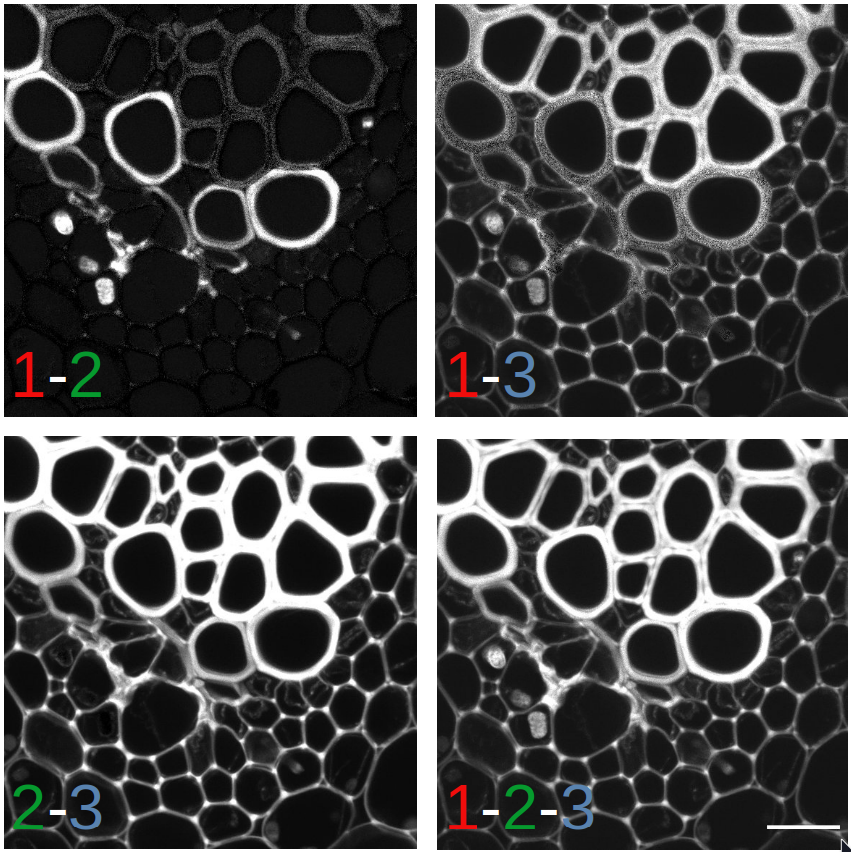
\includegraphics[width=.49\columnwidth]{Exp_3_LSM/Figures/MS3/F2_grey2}}\\
\caption{\textbf{A} (top) is the emission spectra of the individual channels (A~1-3) taken by ACE of the rhizome of a lily of the valley specimen. 
\textbf{B} shows the composites of the combinations of channels, shown here in grey scale for easier comparison. 
Objective lens: Plan Neofluar 20$\times$/0.5. 
Scalebar is 25 $\mu$m.}
\label{fig:autace}
\end{figure}

A linear unmixing method that can be employed to separate fluorescence signals that are close to one another is the Automatic Component Extraction (ACE) in which a Lambda stack is acquired. 
The Lambda stack is a collection of whole images taken with incrementing wavelength ($\pm$10 nm apart.). 
Usually, spectral information are directly searched from the Lambda stack by inspecting all channels for regions within where no signal is detected in the other channels. 
That region is then assigned as pure fluorophore/regarded as reference and can be used for the unmixing operation. 
If such region is not found, then the area with the lowest signal intensity in the other channels is assigned to be a reference.
This is how ACE works and is mathematically based on a Principal Component Analysis (PCA)~\cite{ZeissCamp2}.
In Fig.~\ref{ES} is the resulting ACE of a lily of the valley specimen. 
The reference spectra shows that channel 2 is very similar to channel 3 and most likely does not carry significant information not contained in channel 3, this can indeed be seen by comparing the image acquisition of channel 2 \& 3 (Fig.~\ref{ES}2\&3) that shows the cell walls. 
Whereas channel 1 shows the recognition of different cellular structure (Fig.~\ref{ES}1), probably the chloroplasts. 
Arguably, channel 2 can also be picked in place of channel 3, however the spectrum separation between channel 3 and channel 1 would make it as a better option to be chosen. 
This is further confirmed by the composites in Fig.~\ref{Co} in which the combination of channel 1-2 and channel 1-3 show a relatively similar structures that can be recognized although channel 1-3 gives a better overall picture. 
The combination of channel 2-3 brings no information that is not already contained in channel 1-3. 
The composite of all 3 channels is also presented here as a comparison. 

Another channel produced by this function is the residual channel (not shown) which consist of spectral signals that do not match those in the reference library and hence not assigned, this could be signals that arise from saturated pixels or from high background levels~\cite{ZeissCamp2}. 
Ideally, no signal should be exhibited in this channel. 

Similar result could be achieved by manual selection of regions. 
This is shown in Fig.~\ref{fig:manlinun}. Here two channels (Ch. 11 and 15) out of 32 from the Lambda stack were chosen corresponding to the recorded fluorescence signal at 518 and 557 nm. 
It can be seen that the composite of both these channels already gives a complete picture of the sample when compared to the maximum intensity projection of the acquired lambda stack. 
However, manual selection is very tedious to do. 

\begin{figure}[h!]
\centering
\captionsetup[subfigure]{position=bottom}
\subfloat[Ch. 11 \& 15\label{manc}]{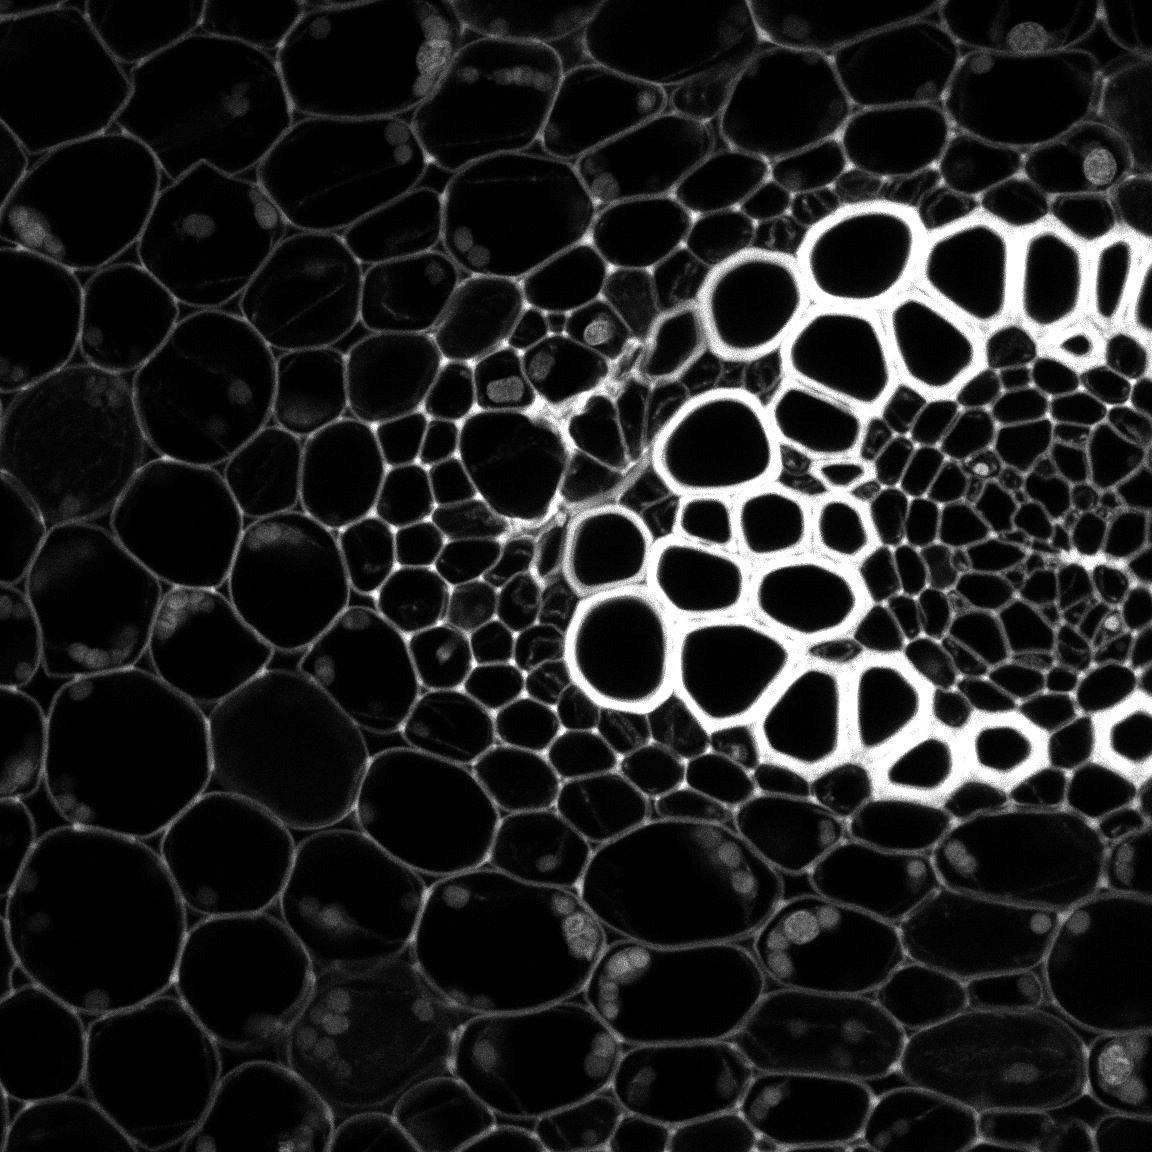
\includegraphics[width=.4\columnwidth]{Exp_3_LSM/Figures/MS3/F2_mipc1115r}}\hspace{0.1mm}
\subfloat[Lambda stack\label{manm}]{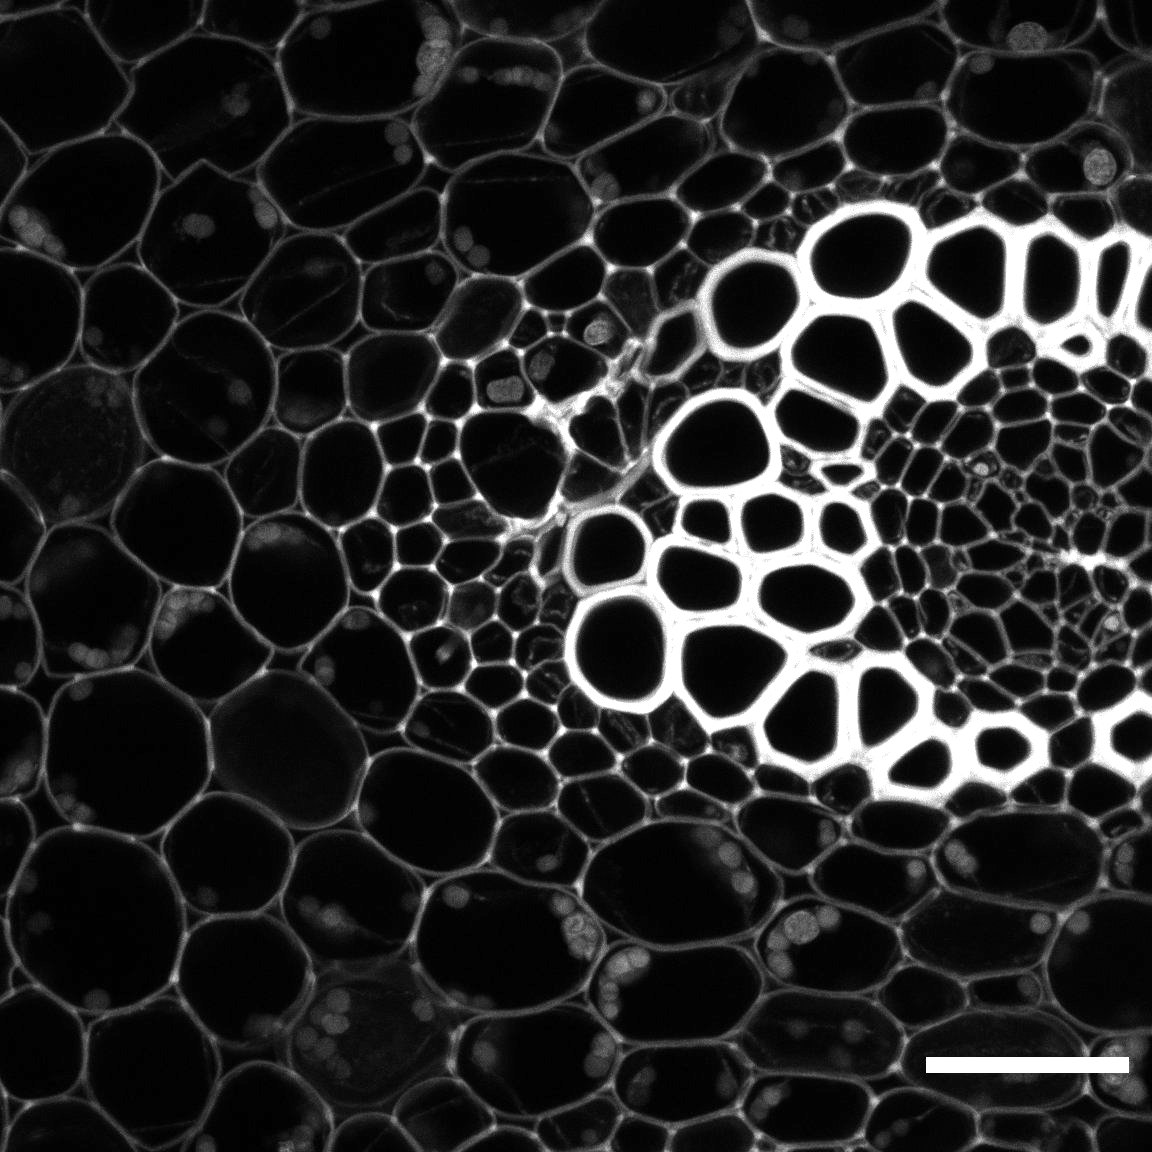
\includegraphics[width=.4\columnwidth]{Exp_3_LSM/Figures/MS3/F2_mipcompr3_50um}}\\
\caption{Manual selection from the Lambda stack. 
Shown here are the maximum intensity projections of: \textbf{A} only Ch. 11 and 15 and \textbf{B} the whole Lambda stack. 
Shown with exaggerated brightness for clarity.  
Objective lens: Plan Neofluar 20$\times$/0.5. 
Scalebar is 50 $\mu$m.} 
\label{fig:manlinun}
\end{figure}

\begin{figure}[h!]
\centering
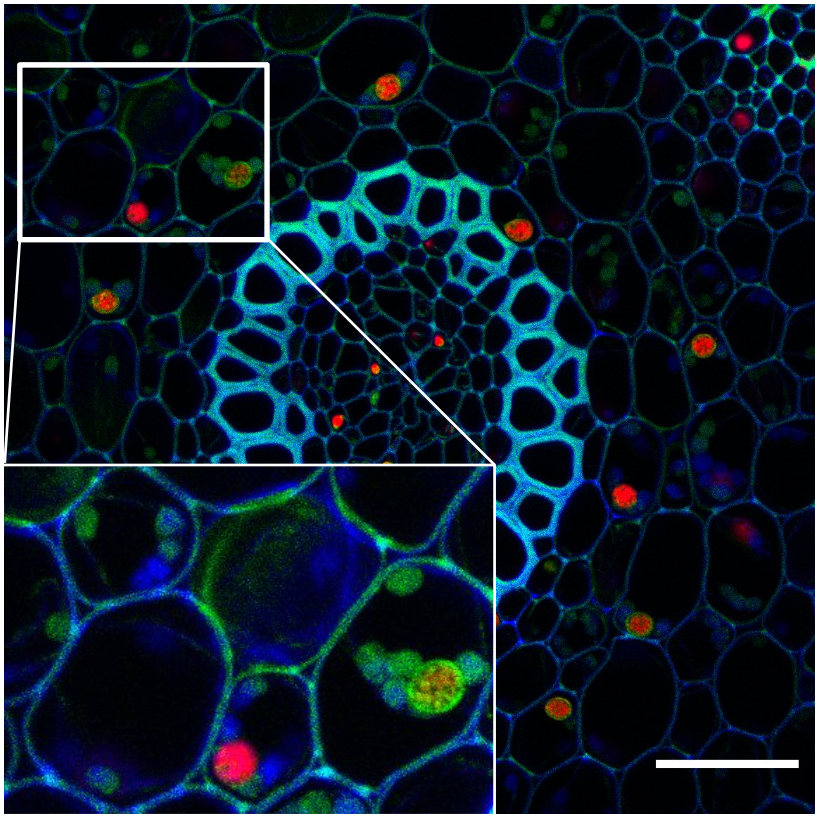
\includegraphics[width=.4\columnwidth]{Exp_3_LSM/Figures/MS3/F2_olfp5_50um}
\caption{Result of using the online fingerprinting function. 
Inset shown with readjusted brightness and constrast. 
Objective lens: Plan Neofluar 20$\times$/0.5. 
Scalebar is 50 $\mu$m.}
\label{fig:olfp}
\end{figure}

The function online fingerprinting was used utilizing the previously acquired result/reference spectra from linear unmixing methods to produce an image shown in Fig.~\ref{fig:olfp}. 
Using this function, the process of separating fluorescence spectral overlap was done during image acquisition. 
In this case, however, it would seem that actually three channels could be appropriate to obtain a complete image as indicated by the inset where a complete image information would not be obtained had one channel be omitted.

\begin{figure}[h!]
\centering
\subfloat[Algae\label{spi}]{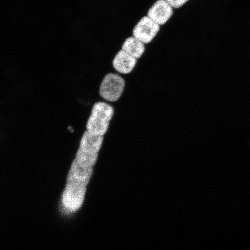
\includegraphics[width=.28\columnwidth]{Exp_3_LSM/Figures/MS3/F3_a}}\hspace{0.1em}
\subfloat[Diatoms\label{dia}]{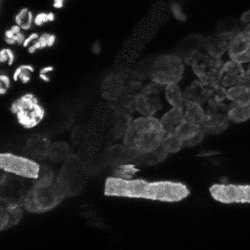
\includegraphics[width=.28\columnwidth]{Exp_3_LSM/Figures/MS3/F3_b}}\hspace{0.1em}
\subfloat[Composite\label{mer}]{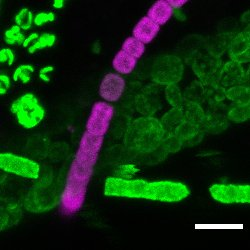
\includegraphics[width=.28\columnwidth]{Exp_3_LSM/Figures/MS3/F3_10um}}\\
\caption{Algae and diatoms autofluorescence. 
Objective lens: C Apochromat 40$\times$/1.2 Imm water immersion. 
Scalebar is 10 $\mu$m.}
\label{fig:diatalg}
\end{figure}

The phenomenon of autofluorescence can be exhibited by a variety of organisms. 
A sample taken from a pond consisting of algae and diatoms shows this behaviour. 
Shown in Fig.~\ref{fig:diatalg} is the autofluorescence of a live sample of algae and diatomes taken from the pond. 
It can be seen here that there are algae that have similar fluorescence spectrum with diatoms and other algae that do not.

\begin{figure}[h!]
\centering
\captionsetup[subfigure]{position=top}
\subfloat[MIP\label{mip}]{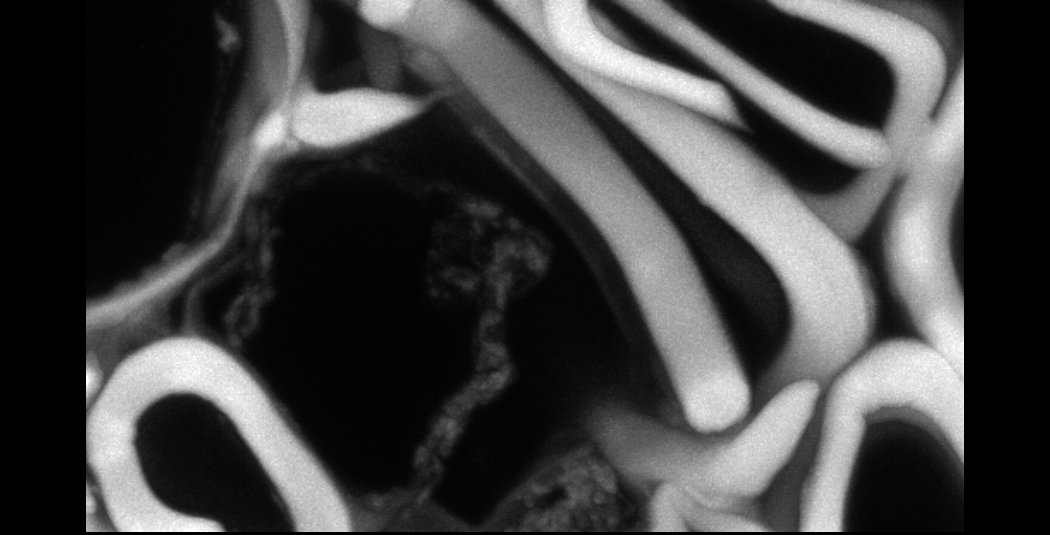
\includegraphics[width=.4\columnwidth]{Exp_3_LSM/Figures/MS3/F4_m}}\hspace{0.1em}
\subfloat[Surface Rendering\label{sur}]{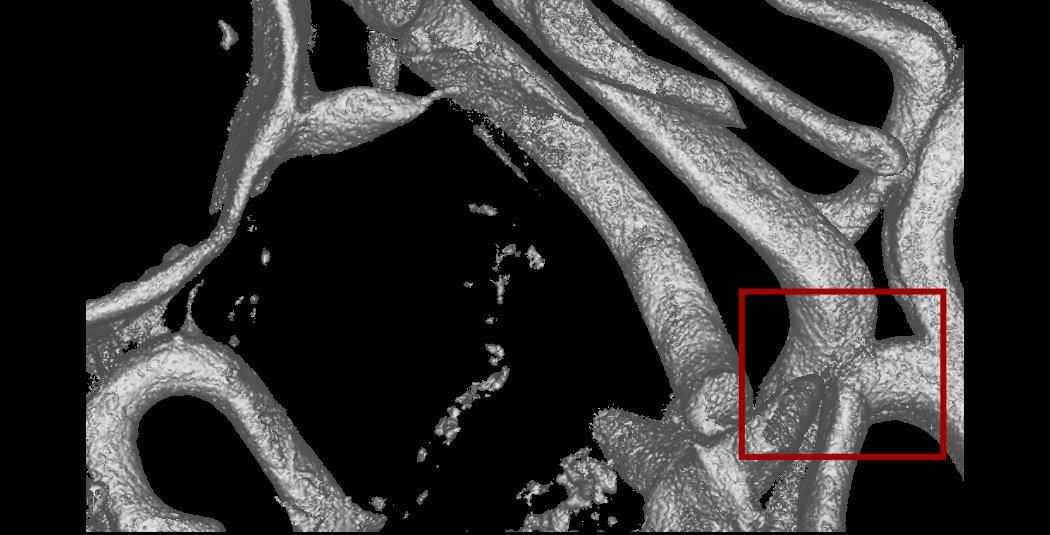
\includegraphics[width=.4\columnwidth]{Exp_3_LSM/Figures/MS3/F4_surred}}\vspace{-0.6em}
\captionsetup[subfigure]{position=bottom}
\subfloat[Depth Coding\label{dep}]{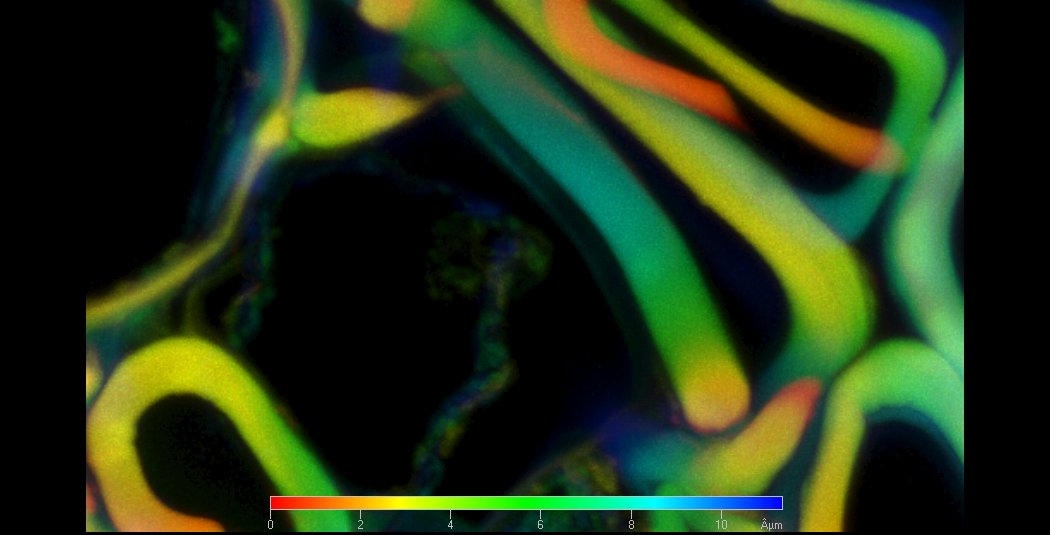
\includegraphics[width=.4\columnwidth]{Exp_3_LSM/Figures/MS3/F4_dep}}	\hspace{0.1em}
\subfloat[Shadow Projection\label{sha}]{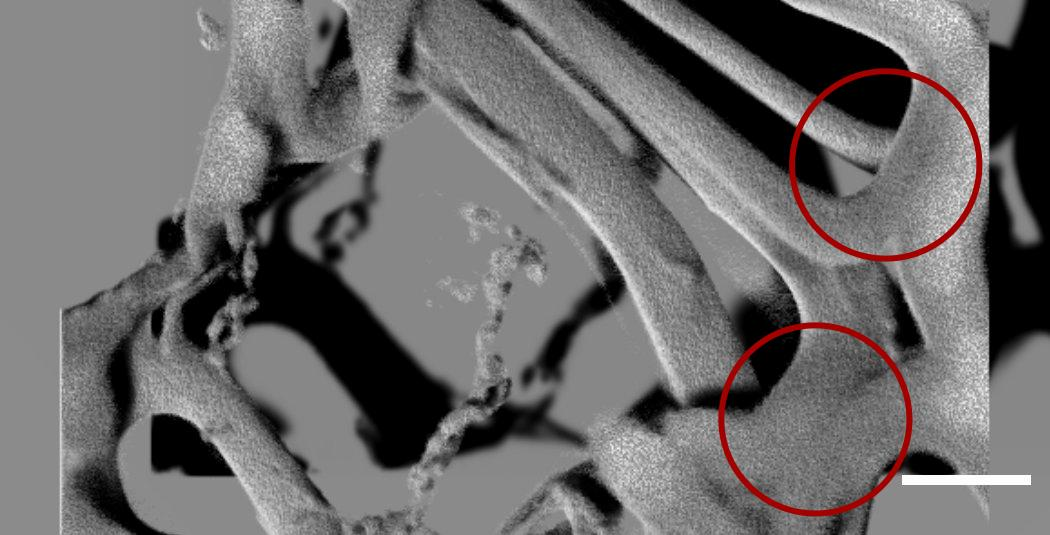
\includegraphics[width=.4\columnwidth]{Exp_3_LSM/Figures/MS3/F4_sha5umred}}\\
\caption{3D representation of a cross section of the rhizome of a lily of the valley specimen. 
Objective lens: Plan Apochromat 63$\times$/1.4 Oil. 
Scalebar is 5 $\mu$m. 
Areas enclosed by red square/circle represent area(s) that are challenging to interpret.} 
\label{fig:3drep}
\end{figure}

As mentioned previously, confocal technique/LSM also allows for imaging a specimen in 3-D. 
Fig.~\ref{fig:3drep} shows a comparison of four representation options of a 3-D image acquisition (z-stack) of the rhizome of a lily of the valley specimen. 
Maximum intensity projection (Fig.~\ref{mip}) is very simple, depth is intuitively recognizeable, and still maintains the sense of 3-D of the structures despite the simplicity. 
It is the most commonly used representation. 
Surface rendering approaches may introduce some texture on the surface of structures which could make recognition difficult as indicated by the red rectangle in Fig.~\ref{sur}. 
Depth coding (Fig.~\ref{dep}) emphasizes in providing depth information, however it is not as simple as maximum intensity projection due to the fact that most of the information is carried by colors (which neccesitates the use of one). 
Depending on the case, some purpose may require the use of this method. Shadow projection offers a strong sense of three-dimentionality, however some parts can be easily obscured as demonstrated by the red circles in Fig.~\ref{sha}. 

\begin{figure}[h!]
\centering
\subfloat[Unadjusted Z-step\label{app}]{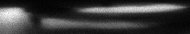
\includegraphics[width=.29\columnwidth]{Exp_3_LSM/Figures/MS3/F4_z11}}\hspace{0.1em}
\subfloat[XY-adjusted Z-step\label{xy}]{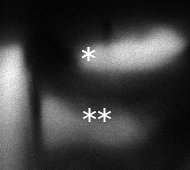
\includegraphics[width=.29\columnwidth]{Exp_3_LSM/Figures/MS3/F4_z22a}}\hspace{0.1em}
\subfloat[Auto-brightness\label{aut}]{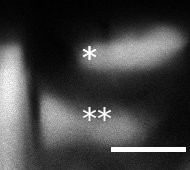
\includegraphics[width=.29\columnwidth]{Exp_3_LSM/Figures/MS3/F4_z33_5uma}}\\
\caption{\textit{Z-section} of the rhizome of a lily of the valley specimen. 
White star symbols shows the comparison of fluoresence signal strength. 
Objective lens: Plan Apochromat 63$\times$/1.4 Oil. 
Scalebar is 5 $\mu$m.} 
\label{fig:zstep}
\end{figure}

A z-section made by the previous image acquisition is shown in Fig.~\ref{app}. 
This presentation shows a rather compressed z-section. 
Applying corrections by adapting the z-step length to the pixel size in x-y, Fig.~\ref{xy} is obtained which shows a more appropriate dimension, although it is apparent that the top part of the specimen receives more excitation and exhibits a stronger fluorescence response. 
Adjusting auto z-brightness correction (Fig.~\ref{aut}) allows for a more evenly distributed signal to deal with the fact that fluorescence response gets weaker the deeper a layer is located. 
This can be seen clearly by inspecting Fig.~\ref{xy} and~\ref{aut} along with the white star symbols as a comparison.

\begin{figure}[h!]
\centering
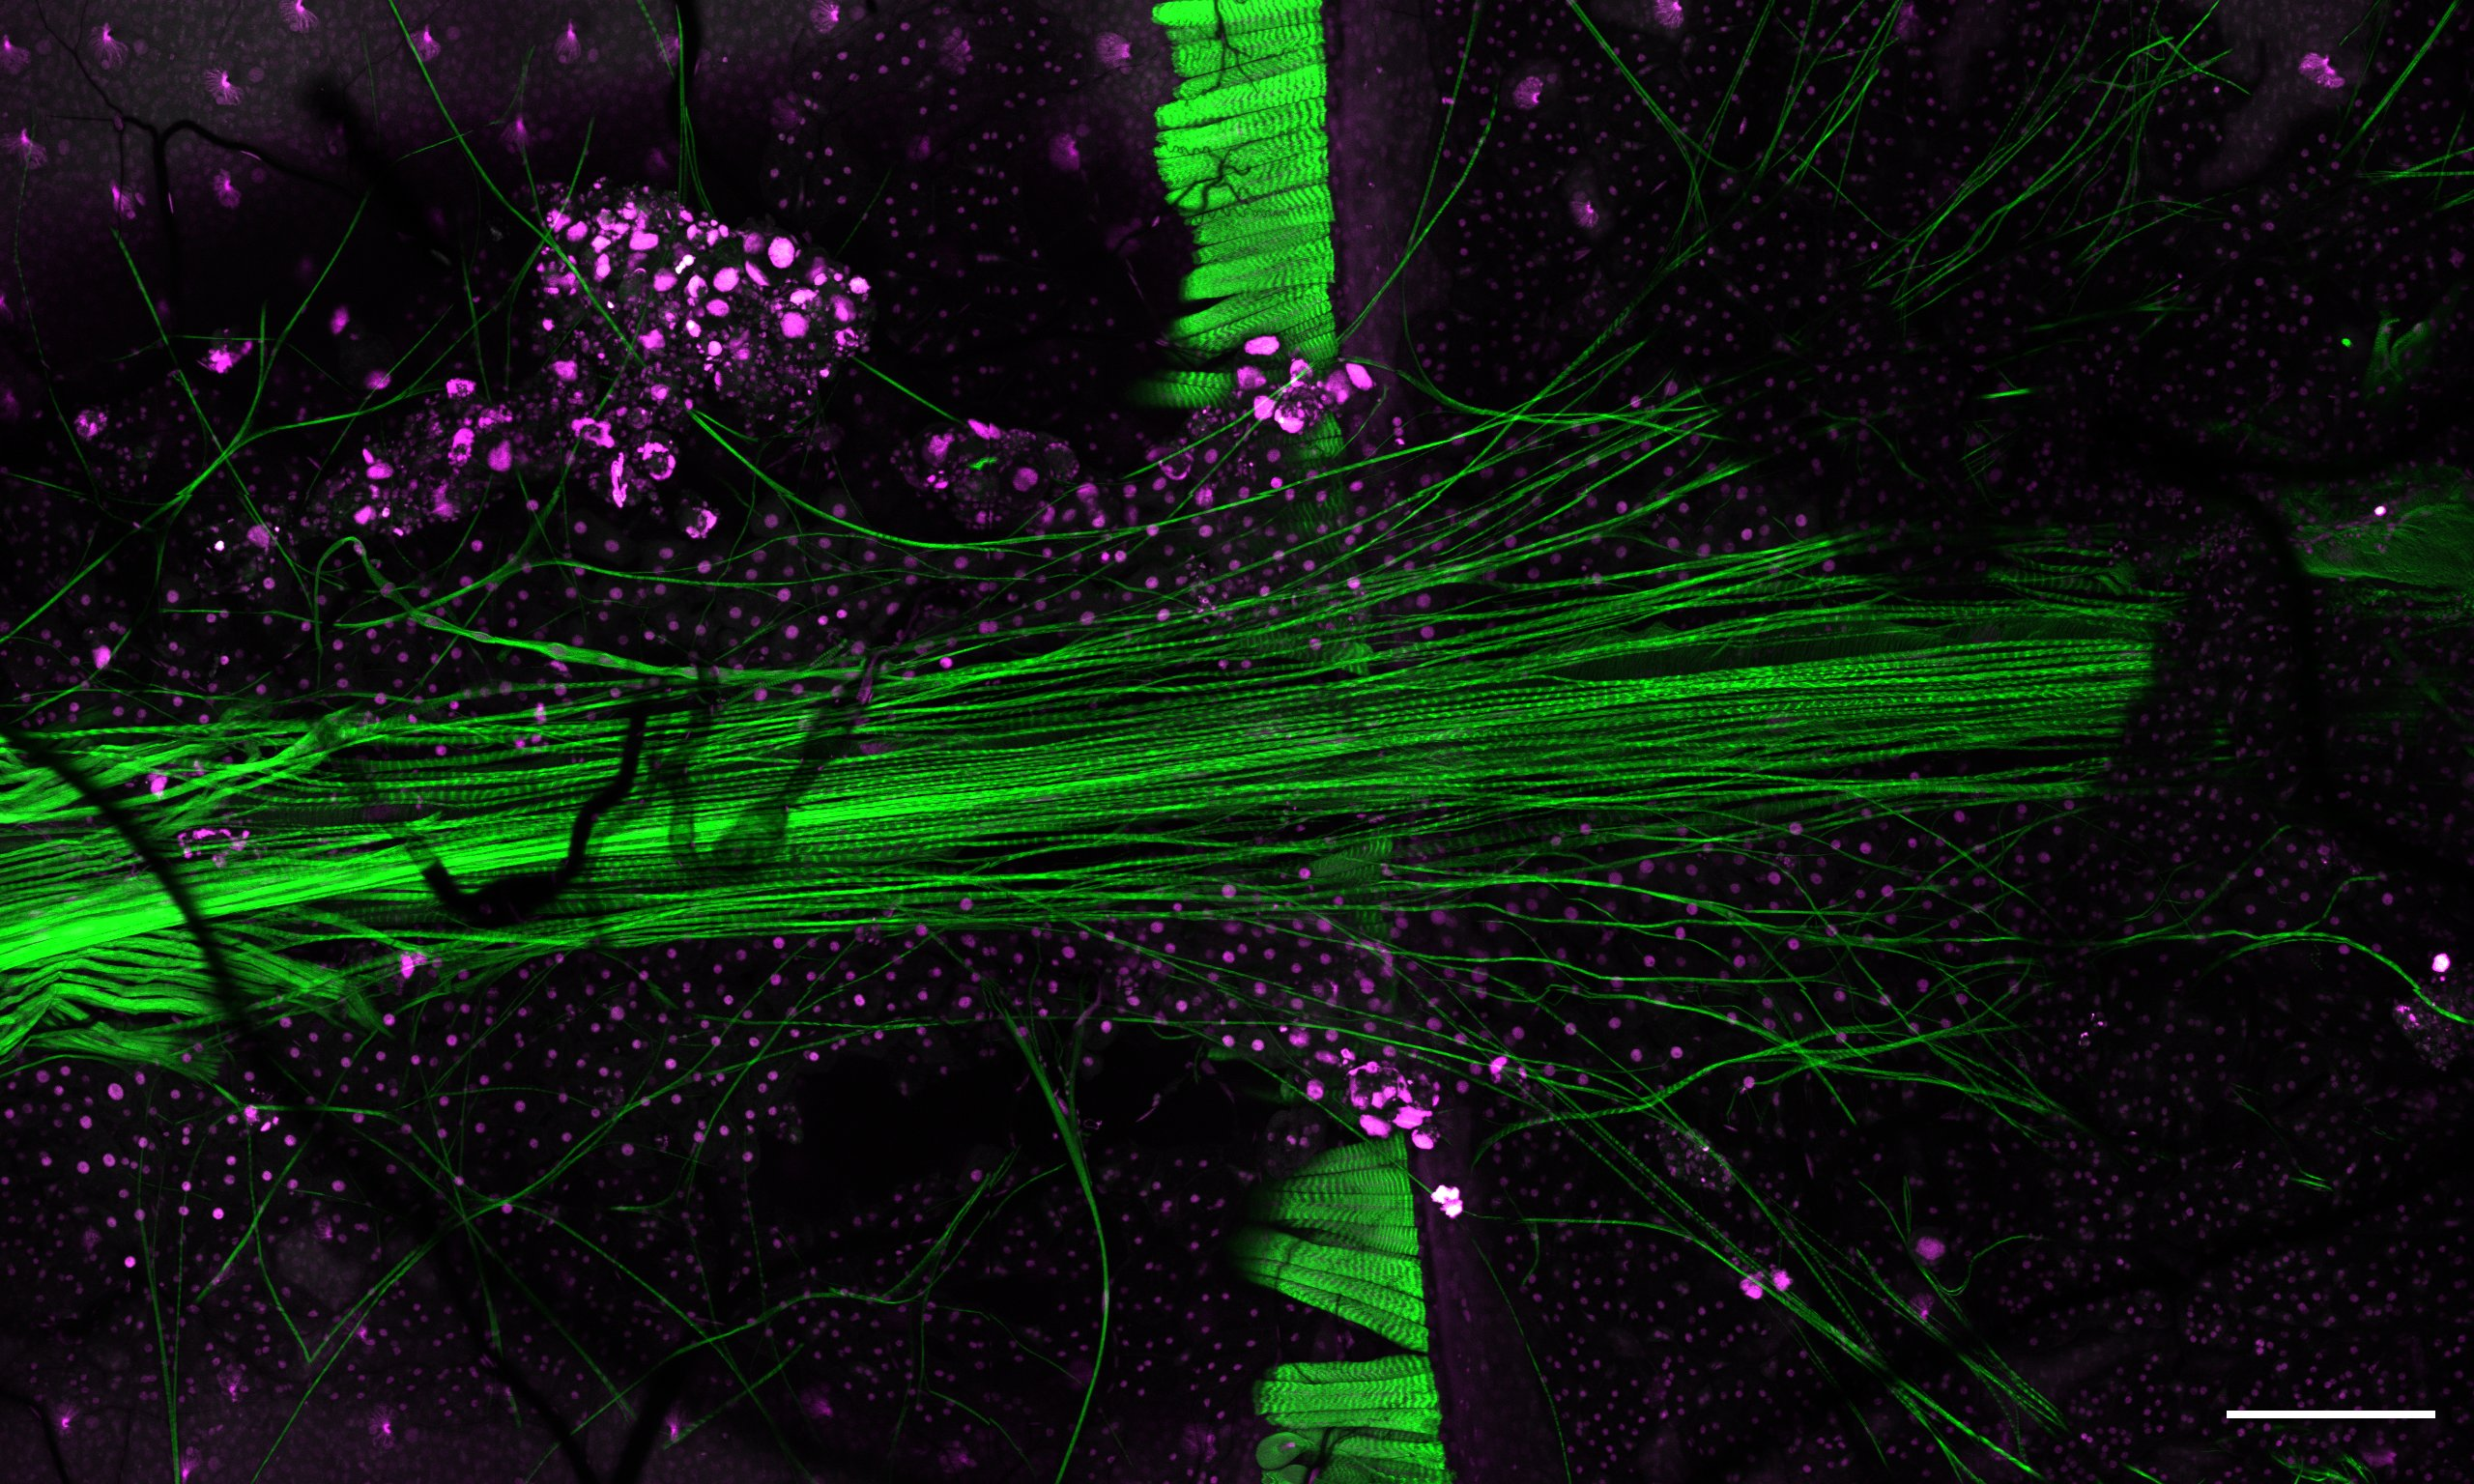
\includegraphics[width=0.8\columnwidth]{Exp_3_LSM/Figures/MS3/F5mg_150um}	
\caption{ A large area of a blowfly abdomen (heart) specimen. 
Green is actin labelled by AlexaFluor 488-Phalloidin, and blue is nucleus labelled by DAPI. 
Objective lens: Plan Neofluar 20$\times$/0.5. 
Scalebar is 150 $\mu$m.}
\label{fig:bloabdo}
\end{figure}

Sometimes, the area one would like to image is larger than the view offered by the device. 
The option \textit{Tile Scan} allows for imaging a large area of a specimen by moving the scan area automatically. 
The acquired large-area image of a blowfly abdomen (heart) is shown in Fig.~\ref{fig:bloabdo}.

\begin{figure}[h!]
\centering
\subfloat[Septate Junctions\label{Fa}]{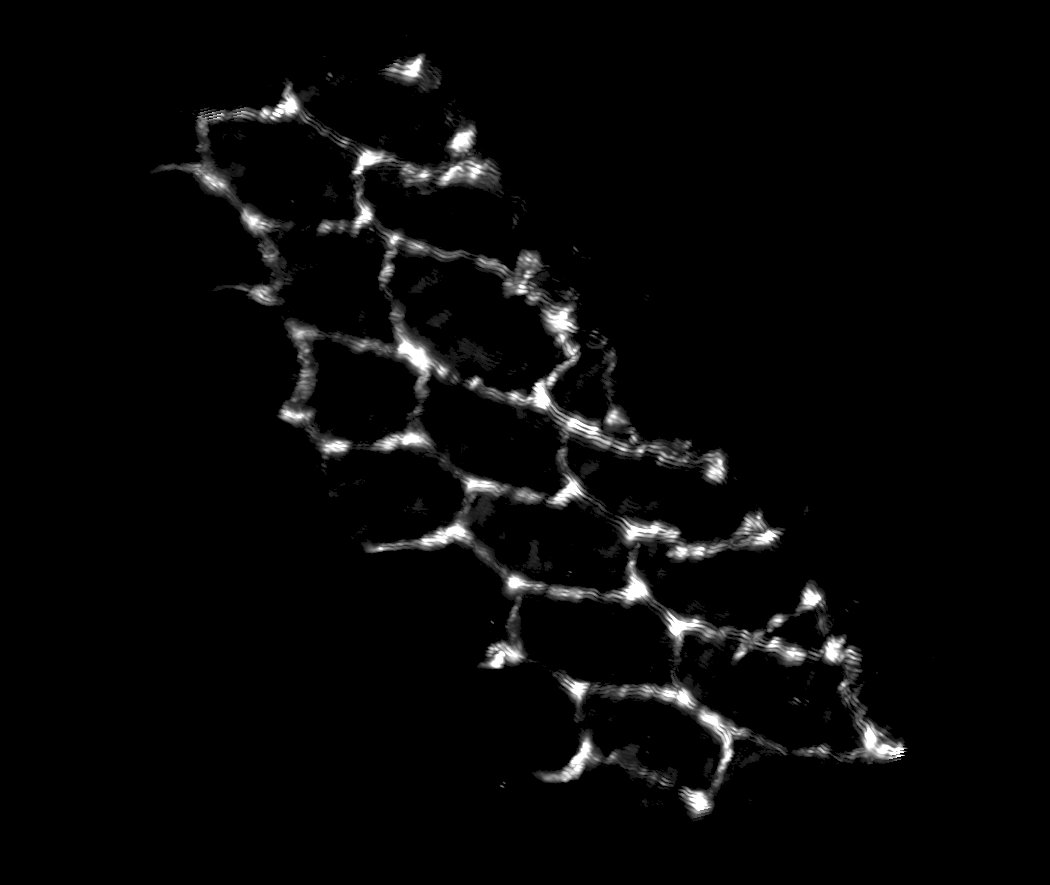
\includegraphics[width=.28\columnwidth]{Exp_3_LSM/Figures/MS3/F6_1}}\hspace{0.1em}
\subfloat[Actin\label{Ac}]{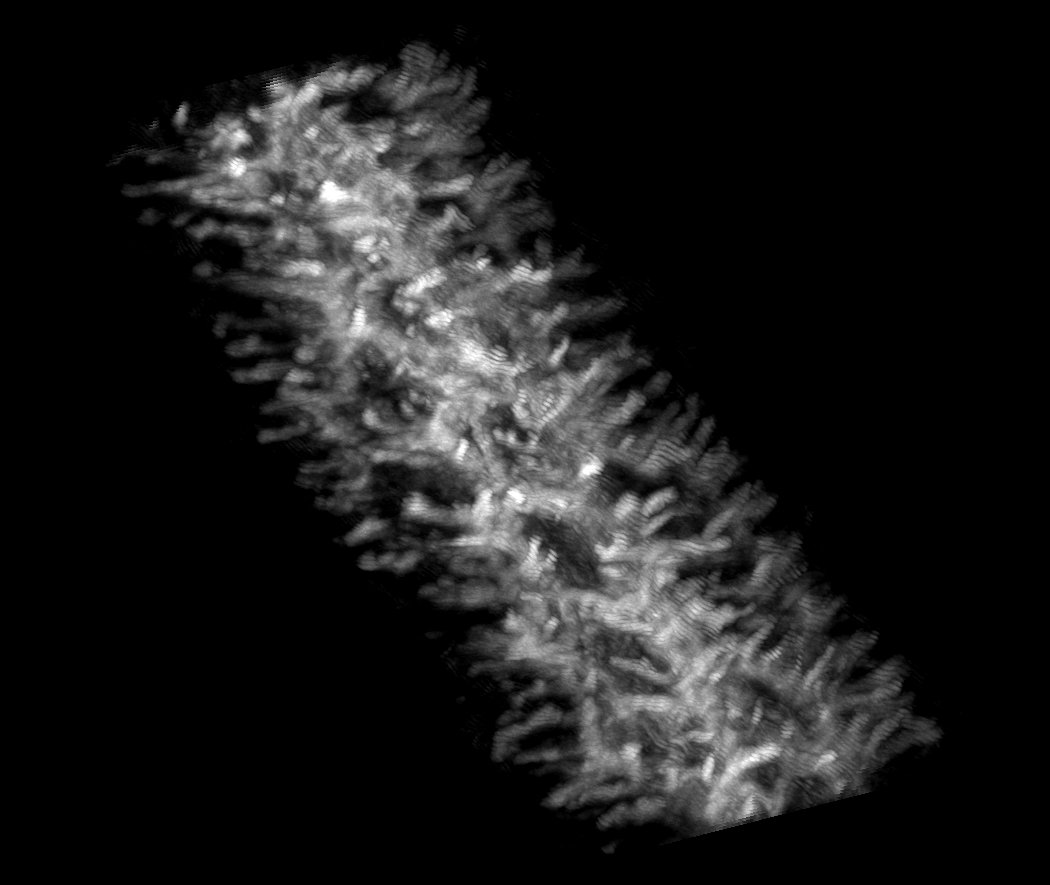
\includegraphics[width=.28\columnwidth]{Exp_3_LSM/Figures/MS3/F6_2}}\hspace{0.1em}
\subfloat[Composite\label{Me}]{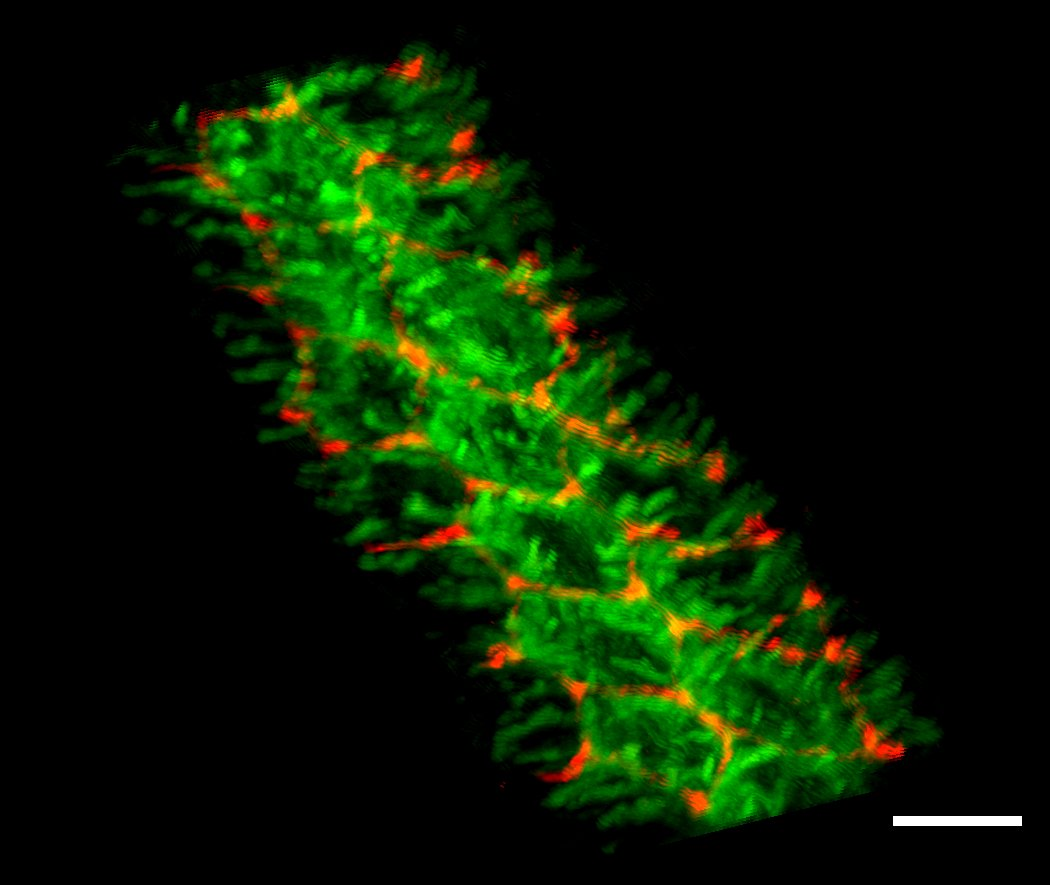
\includegraphics[width=.28\columnwidth]{Exp_3_LSM/Figures/MS3/F6_5um}}\\
\caption{Blowfly salivary gland. 
Septate junctions labelled by AlexaFluor568, actin is labelled by AlexaFluor488. 
Objective lens: C Apochromat 40$\times$/1.2 lmm water immersion. 
Scalebar is 5 $\mu$m.}
\label{fig:what}
\end{figure}

Fig.~\ref{fig:what} shows a 3-D perspective of a z-stack image acquisition of a blowfly salivary gland where Fasciclin-III is labelled by anti-Fasciclin-III/AlexaFluor568-conjugated goat anti-mouse-IgG, actin is labelled by AlexaFluor488, and nucleus is labelled by DAPI, which is not visible perhaps due to the possibility that the nucleus has diffused out of the sample because the sample is old. 

The pinhole size of a confocal microscopy affects not only in the xy-dimension, but also the resolution in the z-dimension, as can be seen in Fig.~\ref{fig:goldpin} that shows xz-section of a gold-covered coverslip, where the smaller pinhole size gives a better resolved image. 
This is confirmed as well by the calculation of the FWHM of the acquisitions where the FWHM increases along with the increasing pinhole opening size. 
The FWHM calculation was done by a gaussian fit to the intensity-distance data of the acquisitions of each pinhole size with neither intensity normalization nor baseline corrections. 
To note, the data for pinhole opening of 3 AU seems to be jeopardized, and hence excluded from calculation. 

\begin{figure}[h!]
\centering
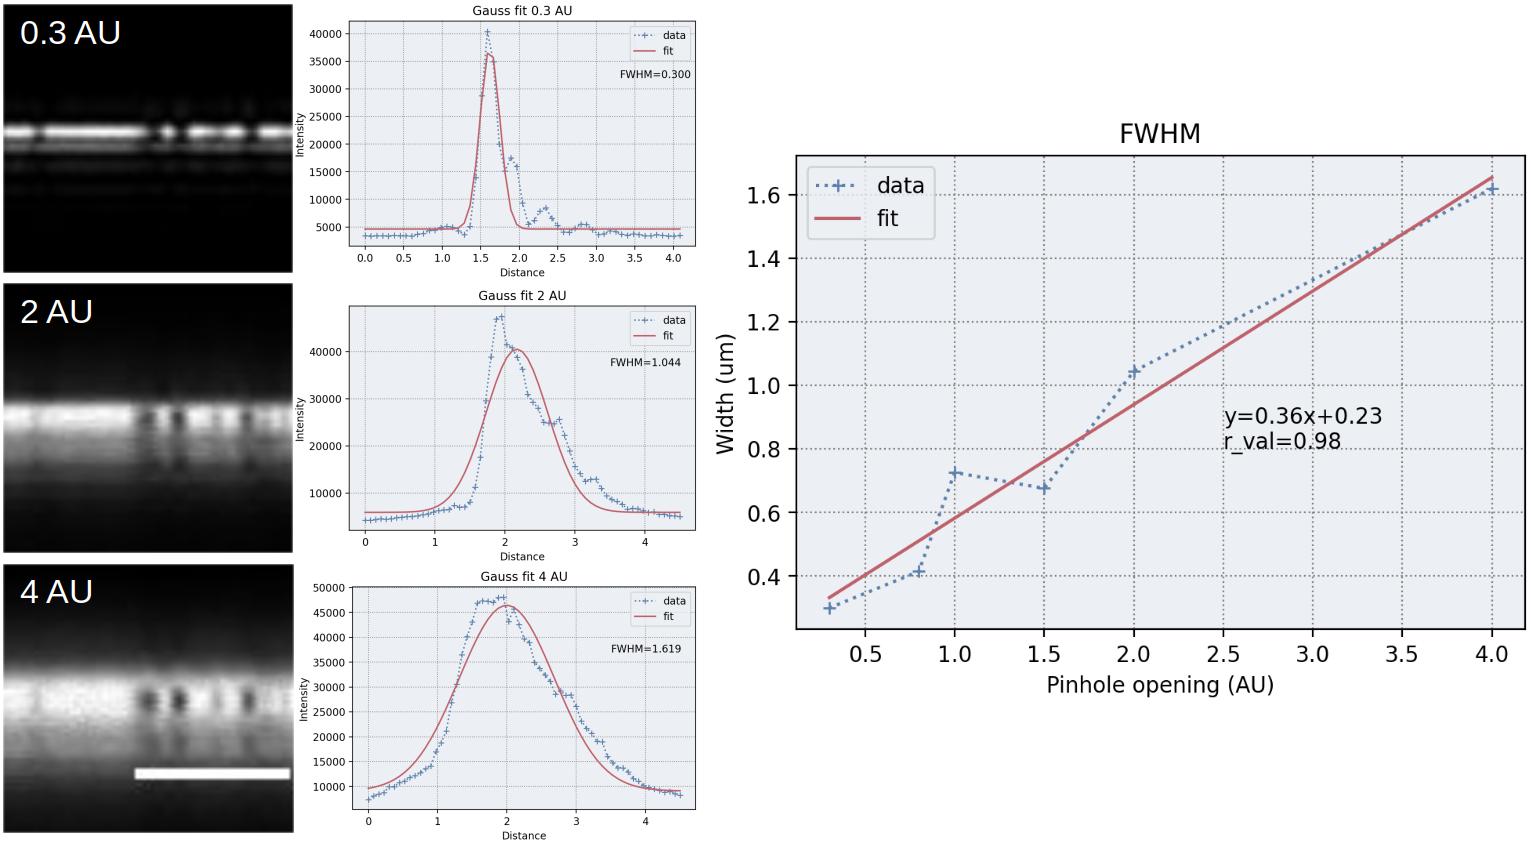
\includegraphics[width=.9\columnwidth]{Exp_3_LSM/Figures/MS3/F7a}	
\caption{xz-section of a gold-covered coverslip with different pinhole sizes along with the gaussian fit to obtain the FWHM, and the relationship between it and pinhole sizes. 
Images were acquired with pinhole size 0.3, 0.8, 1, 1.5, 2, and 4 AU (here shown only a selection of those). 
Objective lens: Plan Apochromat 63$\times$/1.4 Oil. 
Scalebar is 3 $\mu$m.}
\label{fig:goldpin}
\end{figure}


%----------------------------------------------------------------------------------------
%	BIBLIOGRAPHY
%----------------------------------------------------------------------------------------

\renewcommand{\refname}{\spacedlowsmallcaps{References}} % For modifying the bibliography heading

%\bibliographystyle{unsrt}

%\bibliography{sample.bib} % The file containing the bibliography

